% 
%            ,,                                        
%          `7MM            _.o9                                
%            MM                                             
%  ,6"Yb.    MM  ,p6"bo   ,6"Yb.  M"""MMV  ,6"Yb.  `7Mb,od8 
% 8)   MM    MM 6M'  OO  8)   MM  '  AMV  8)   MM    MM' "' 
%  ,pm9MM    MM 8M        ,pm9MM    AMV    ,pm9MM    MM     
% 8M   MM    MM YM.    , 8M   MM   AMV  , 8M   MM    MM     
% `Moo9^Yo..JMML.YMbmd'  `Moo9^Yo.AMMmmmM `Moo9^Yo..JMML.   
% 
% 
% Free and Open-Source template for academic works
% https://github.com/dpmj/alca



\clearpage
\cleardoublepage

\chapter{Problemi bioinformatici ad alta complessità}

La \glsname{bioinf}, disciplina interdisciplinare congiungente biologia e informatica, ha conosciuto un rapido sviluppo negli ultimi decenni grazie alla crescente disponibilità di dati biologici ad alta dimensionalità. La disciplina si propone di analizzare, interpretare e gestire le informazioni biologiche mediante l'impiego di strumenti computazionali avanzati. Tale ambito ha preso piede in virtù della sua capacità di contribuire significativamente alla comprensione dei fenomeni biologici complessi. La bioinformatica abbraccia molteplici sfaccettature, tra cui l'analisi del genoma, la proteomica, la trascrittomica e la metabolomica, fornendo un quadro completo delle intricazioni biologiche che costituiscono il fondamento della vita.

Parallelamente, l'introduzione del \glsname{ml} nella bioinformatica ha rappresentato una svolta epocale, consentendo l'analisi efficiente di grandi dataset biologici \cite{lecun2015deep, angermueller2016deep}. Modelli di machine learning, quali reti neurali, support vector machines e algoritmi di apprendimento profondo, sono stati impiegati per identificare pattern nascosti nei dati biologici, predire interazioni molecolari, classificare malattie genetiche e persino progettare nuove molecole farmaceutiche. Studi come quelli condotti da Ching et al. \cite{ching2018deep} e Min et al. \cite{min2017deep} attestano la crescente efficacia dell'approccio ML nell'affrontare questioni complesse in ambito bioinformatico.

Tuttavia, l'applicazione di modelli di machine learning alla bioinformatica non è priva di sfide intrinseche. La complessità e la variabilità dei dati biologici, la presenza di rumore sperimentale e la necessità di interpretare risultati in un contesto biologico rendono ardua l'adozione di modelli standard. Inoltre, la carenza di dataset sufficientemente ampi e ben etichettati rappresenta un ostacolo alla creazione di modelli generalizzabili. Pubblicazioni quali quelle di Ching et al. \cite{ching2018deep} e Min et al. \cite{min2017deep} evidenziano le difficoltà incontrate nel bilanciare precisione e generalizzazione nella pratica bioinformatica attraverso l'utilizzo di modelli di machine learning. La continua ricerca e lo sviluppo di nuovi approcci e metodologie sono dunque imperativi per superare tali sfide e massimizzare il potenziale della bioinformatica nell'era dell'informazione molecolare.

Un uilteriore esempio notevole dell'applicazione del machine learning in bioinformatica è l'uso di \glsname{nn} per predire la struttura tridimensionale delle proteine. La ricerca di Senior et al. (2020) ha dimostrato progressi significativi in questo ambito \cite{senior2020improved}.

\section{I modelli GeneFusion}

Questa tesi itera su un lavoro accademico predentemente realizzato dagli studenti Antonio Cirillo ed Eugenio De Simone dell'Università degli Studi di Salerno \cite{cirillo} \cite{desimone}, supervisionati dal relatore Rocco Zaccagnino.

Gli studenti hanno avanzato uno spettro di analisi e sperimentazioni legate alla classificazione dei geni e all'individuazione delle cosiddette reads chimeriche, motivate dall'alta presenza di falsi positivi negli strumenti di classificazione dei geni di fusione. In generale, gli studenti hanno suggerito una scarsa qualità delle classificazioni dei tool pre-esistenti, suggerendo dunque la necessità di produrne dei nuovi. Nel tentativo di affrontare queste limitazioni, gli studenti hanno proposto nuovi strumenti basate su tecniche di \glsname{dl} in grado di contribuire all'individuamento di reads chimeriche in pazienti affetti da condizioni sensibili quali la leucemia linfoblastica acuta. Per studiare l'efficienza e l'efficacia della soluzione proposta, sono state condotte ulteriori sperimentazioni confrontando il tool realizzato con altrimenti strumenti ben noti come {\em FusionCatcher}. Gli studenti hanno, infine, osservato che le tecniche di deep learning hanno effettivamente svolto un ruolo centrale nel migliorare i tool pre-esistenti, specialmente per le fasi di sequenziamento ed allineamento.

I modelli {\em Gene Classifier} e {\em Fusion Classifier} (che, insieme, rappresentano i "modelli GeneFusion"), sviluppati in ottica open-source e disponbili pubblicamente su GitHub \cite{kubeless_gf}, sfruttano tecnologie ben note come Python, PyTorch, Numpy e Pandas, per le quali si rimanda alle rispettive documentazioni ufficiali; inoltre, gli studenti hanno adoperato ulteriori tecnologie ausiliarie, come Fusim \cite{fusim} e GenomeTools \cite{gt}.

La repository di GeneFusion ha la seguente forma:

\begin{small}
\begin{Verbatim}[commandchars=\\\{\}]
    \textcolor{blue}{antoniogrv@linux} \textcolor{blue!50}{ ~/kubeless-gf $} ls
    data         model             tokenizer          utils
    dataset      README.md         \textcolor{purple!80}{train_gene_classifier.py}
    grid_search  \textcolor{gray}{requirements.txt}  \textcolor{purple!80}{train_fusion_classifier.py}
\end{Verbatim}
\end{small}

Gli script di esecuzione {\small {\color{purple!80} \verb|train_gene_classifier.py|}} e {\small {\color{purple!80} \verb|train_fusion_classifier.py|}} eseguono rispettivamente le pipeline di machine learning dei modelli {\em Gene Classifier} e {\em Fusion Classifier}. E' possibile eseguire i due modelli in maniera del tutto indipendente, e raccogliere i frutti del loro output nella stessa directory di esecuzione. Analogamente, è banale osservare come ambo i modelli condividano, allo stato attuale, le stesse dipendenze Python, declinate nel file {\small {\color{gray} \verb|requirements.txt|}}, nonché in generale l'intero filesystem indicato in precedenza. Le cartelle, infatti, contengono moduli Python utilizzati in varie misure nell'esecuzione di ambo i modelli. Si fa notare come, però, alcuni di questi moduli vengano impiegati esclusivamente per uno dei due modelli. In generale, la coesistenza dei modelli nella directory così come presentata suggerisce una forte correlazione fra le pipeline.

\begin{figure}[h]
    \centering
    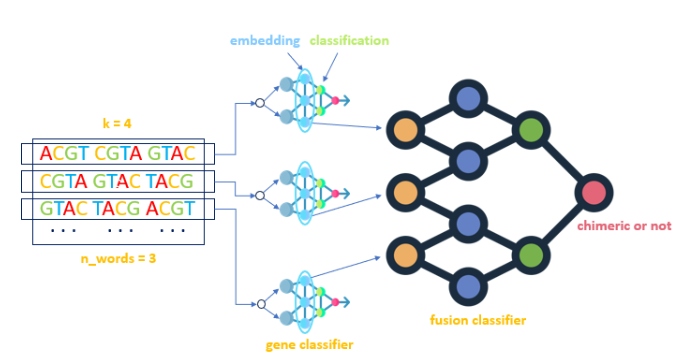
\includegraphics[width=375px]{figures/ch2/genefusion.png}
    \caption[Pipeline di esecuzione dei modelli GeneFusion]{Pipeline di esecuzione dei modelli GeneFusion}
    \label{fig:cha2:gf}
\end{figure}

Tale correlazione è immediatamente individuabile nel file {\small {\color{purple!80} \verb|train_fusion_classifier.py|}}, il quale - una volta captati gli argomenti di esecuzione dello script Python - invoca l'intera pipeline del modello {\em Gene Classifier} prima di procedere all'esecuzione della propria pipeline.

\begin{code}
\captionof{listing}{Fusion Classifier sub-pipeline}
\label{code:apx:a:python}
\begin{minted}{python}
if __name__ == '__main__':
    # define inputs for this script
    __args, __gc_hyperparameters, __hyperparameters = define_fusion_classifier_inputs()

    # load dotenv file
    load_dotenv(dotenv_path=os.path.join(os.getcwd(), '.env'))

    # execute train_gene_classifier method
    train_fusion_classifier(
        **__args,
        gc_hyperparameters=__gc_hyperparameters,
        fc_hyper_parameters=__hyperparameters
)

def train_fusion_classifier(
    len_read: int,
    len_kmer: int,
    n_words: int,
    tokenizer_selected: str,
    n_fusion: int,
    gc_model_selected: str,
    gc_hyperparameters: Dict[str, any],
    gc_batch_size: int,
    gc_re_train: bool,
    model_selected: str,
    fc_hyper_parameters: Dict[str, any],
    batch_size: int,
    freeze: bool,
    re_train: bool,
    grid_search: bool,
):
    # execute train_gene_classifier
    gc_model_path, gc_model_config = train_gene_classifier(
        len_read=len_read,
        len_kmer=len_kmer,
        n_words=n_words,
        tokenizer_selected=tokenizer_selected,
        model_selected=gc_model_selected,
        hyper_parameters=gc_hyperparameters,
        batch_size=gc_batch_size,
        re_train=gc_re_train,
        grid_search=True
    )
\end{minted}
\end{code}

Nel codice soprastante, con l'acronimo {\small \verb|gc|} ci si riferisce al modello Gene Classifier. La pipeline del modello Fusion Classifier viene eseguita esclusivamente dopo una run completa della pipeline del modello Gene Classifier.

E' quindi possibile interpretare il modello Fusion Classifier come dipendente dal modello Gene Classifier; il primo adopera il secondo come sotto-modello, sfruttandolo per configurare la propria pipeline come segue.

\begin{code}
\label{code:apx:a:python}
\begin{minted}{python}
model_config: Optional[MyModelConfig] = None

if model_selected == 'fc':
    model_config = FCFullyConnectedModelConfig(
        gene_classifier_name=gc_model_selected,
        gene_classifier_path=gc_model_path,
        n_sentences=n_sentences,
        freeze=freeze,
        **fc_hyper_parameters
    )
elif model_selected == 'rnn':
    model_config = FCRecurrentNNConfig(
        gene_classifier_name=gc_model_selected,
        gene_classifier_path=gc_model_path,
        n_sentences=n_sentences,
        freeze=freeze,
        **fc_hyper_parameters
    )
\end{minted}
\end{code}

Successivamente, {\small \verb|model_config|} verrà adoperato in circa ogni segmento della pipeline di Fusion Classifier. Si sottolinea che, tralasciando questa specifica inter-dipendenza, i modelli si comportano macroscopicamente in modo del tutto analogo, sebbene sfruttino moduli e strumenti diversi.

In ogni caso, ambo i modelli possono essere rappresentati da una macchina a stati che, sequenzialmente, produce i dati richiesti dalle fasi di training e testing, allena e realizza il modello e lo sottopone ad un test di forecasting. Nella fattispecie, vengono realizzati dataset di {\em training}, {\em validation} e {\em testing}. I primi due dataset sono coinvolti nella fase di training, mentre esclusivamente l'ultimo viene coinvolto nella fase di testing. La fase di testing sussegue la fase di training.

\subsection{Il modello Gene Classifier}

\begin{figure}[h]
    \centering
    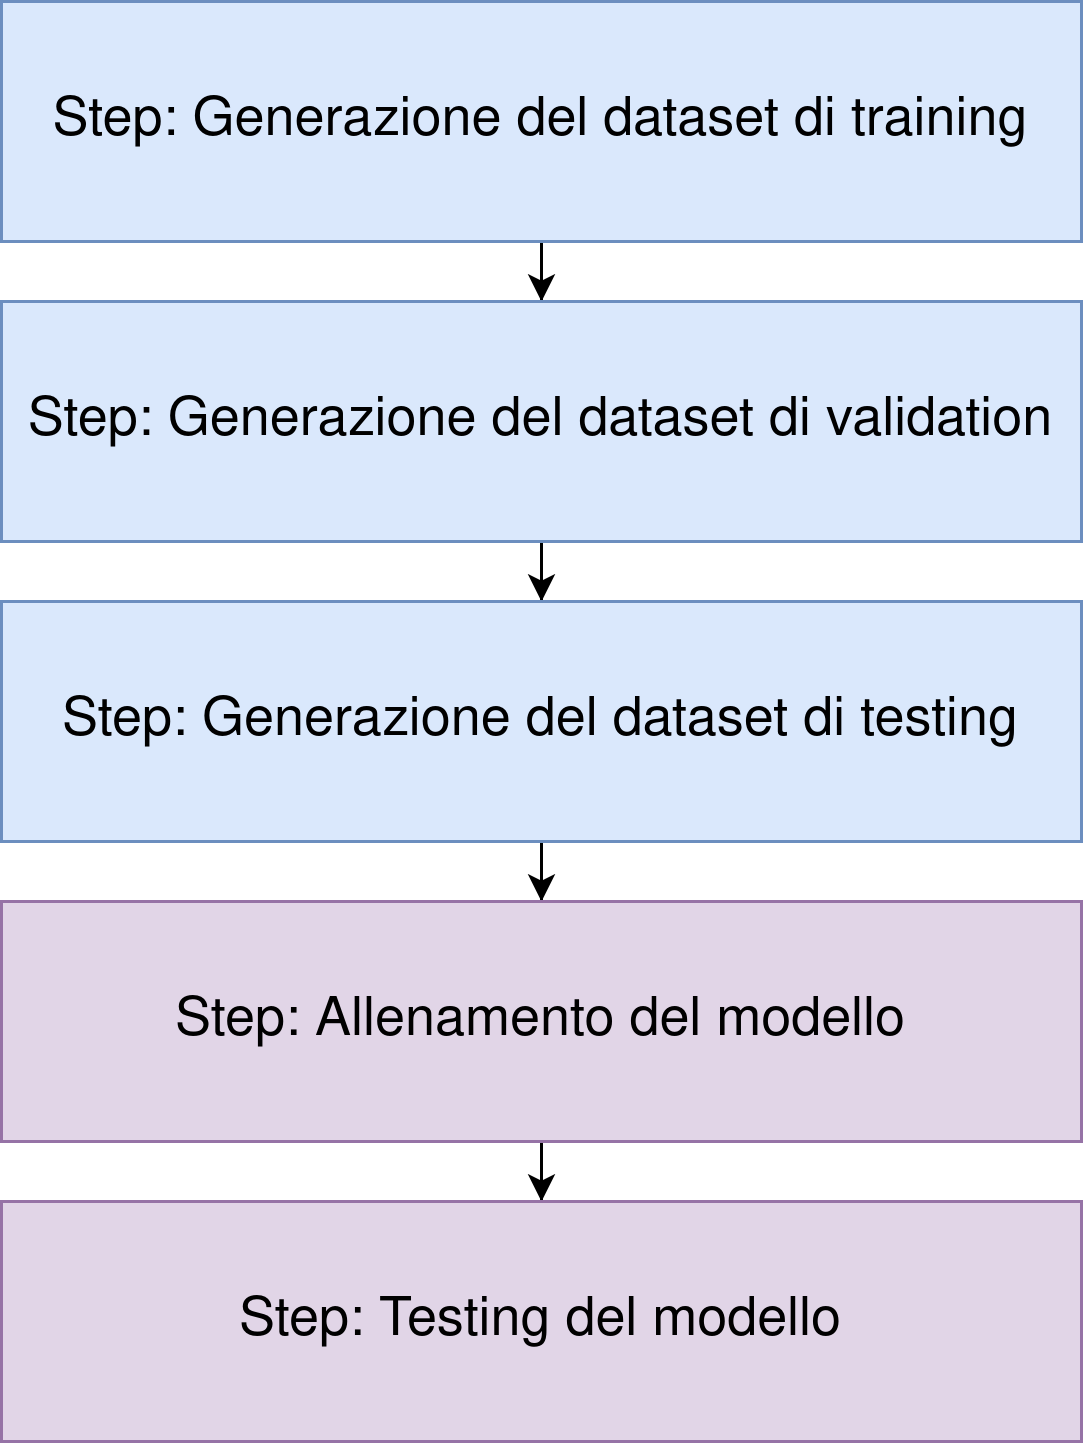
\includegraphics[width=150px]{figures/ch2/gene_stati.png}
    \caption[Sequenza di operazioni del modello Gene Classifier]{Sequenza di operazioni del modello Gene Classifier}
    \label{fig:cha2:gene_stati}
\end{figure}

Come specificato in \cite{cirillo} e \cite{desimone}, il modello Gene Classifier ha, come suggerisce il nome, l'obiettivo di classificare i geni forniti in input. Il modello viene addestrato su un insieme di geni  indicati in un file testuale ({\small \verb|data/genes_panel.txt|}), come {\small \verb|RUNX1, ETV6, RIPOR1, CTCF|} e {\small \verb|KMT2A|}. La selezione dei geni è cruciale per assicurare un comportamento organico e completo del modello, e dovrebbe essere guidata dalla specifica domanda di ricerca e dalle sequenze finali su cui si intende verificare la presenza di geni di fusione. In sintesi, è importante selezionare i geni rilevanti per il contesto di studio. Per ognuno dei geni indicati nel file, uno script Python automatizza il download (da una banca dati esterna) di sequenze genomiche suddivise fra sequenze fusionate e non fusionate. I risultati di questa fase saranno poi disponibili nella directory {\small \verb|data|}.

In particolare, la banca dati a cui ci si rifersce è esposta da un'API di Enembl, che permette di scaricare i trascritti di riferimento dei geni selezionati. L'API interrogherà a sua volta il proprio database per distribuire opportunamente le annotazioni del genoma richiesto. Questo approccio permette di automatizzare completamente la fase di ottenimento dei dati. Ottenuti i dati, il sistema procede come segue:

\begin{enumerate}
    \item Generazione delle sequenze a partire dai trascritti scaricati. Questa fase produce le sequenze interessate che saranno poi usate dalle successive operazioni.
    \item Generazione del file CSV contenente tutti i {\em k-mers} delle sequenze generate al passaggio precedente, inclusive di un'etichetta per identificare il gene di provenienza. Questo file rappresenta l'input per l'addestramento del modello.
    \item Il file CSV viene diviso in tre dataset: training (80\%), testing (10\%) e validation (10\%).
    \item Generazione di tutte le possibili "sentenze" per ogni dataset. Le sentenze sono stringhe di k-mer consecutivi separati da uno spazio. Questa rappresentazione permette di fornire un ulteriore input al modello. I risultati vengono salvati in file distinti, che saranno poi dati in input al modello in fase di training e testing.
    \item Prima di procedere al training e al testing, i valori di input vengono opportunamente tokenizzati usando un vocabolario specifico, chiamato {\em DNA Tokenizer}.
\end{enumerate}

Descrizioni più dettagliate delle fasi soprastanti sono disponibili nei lavori originali citati in precedenza.

\subsection{Il modello Fusion Classifier}
\begin{figure}[h]
    \centering
    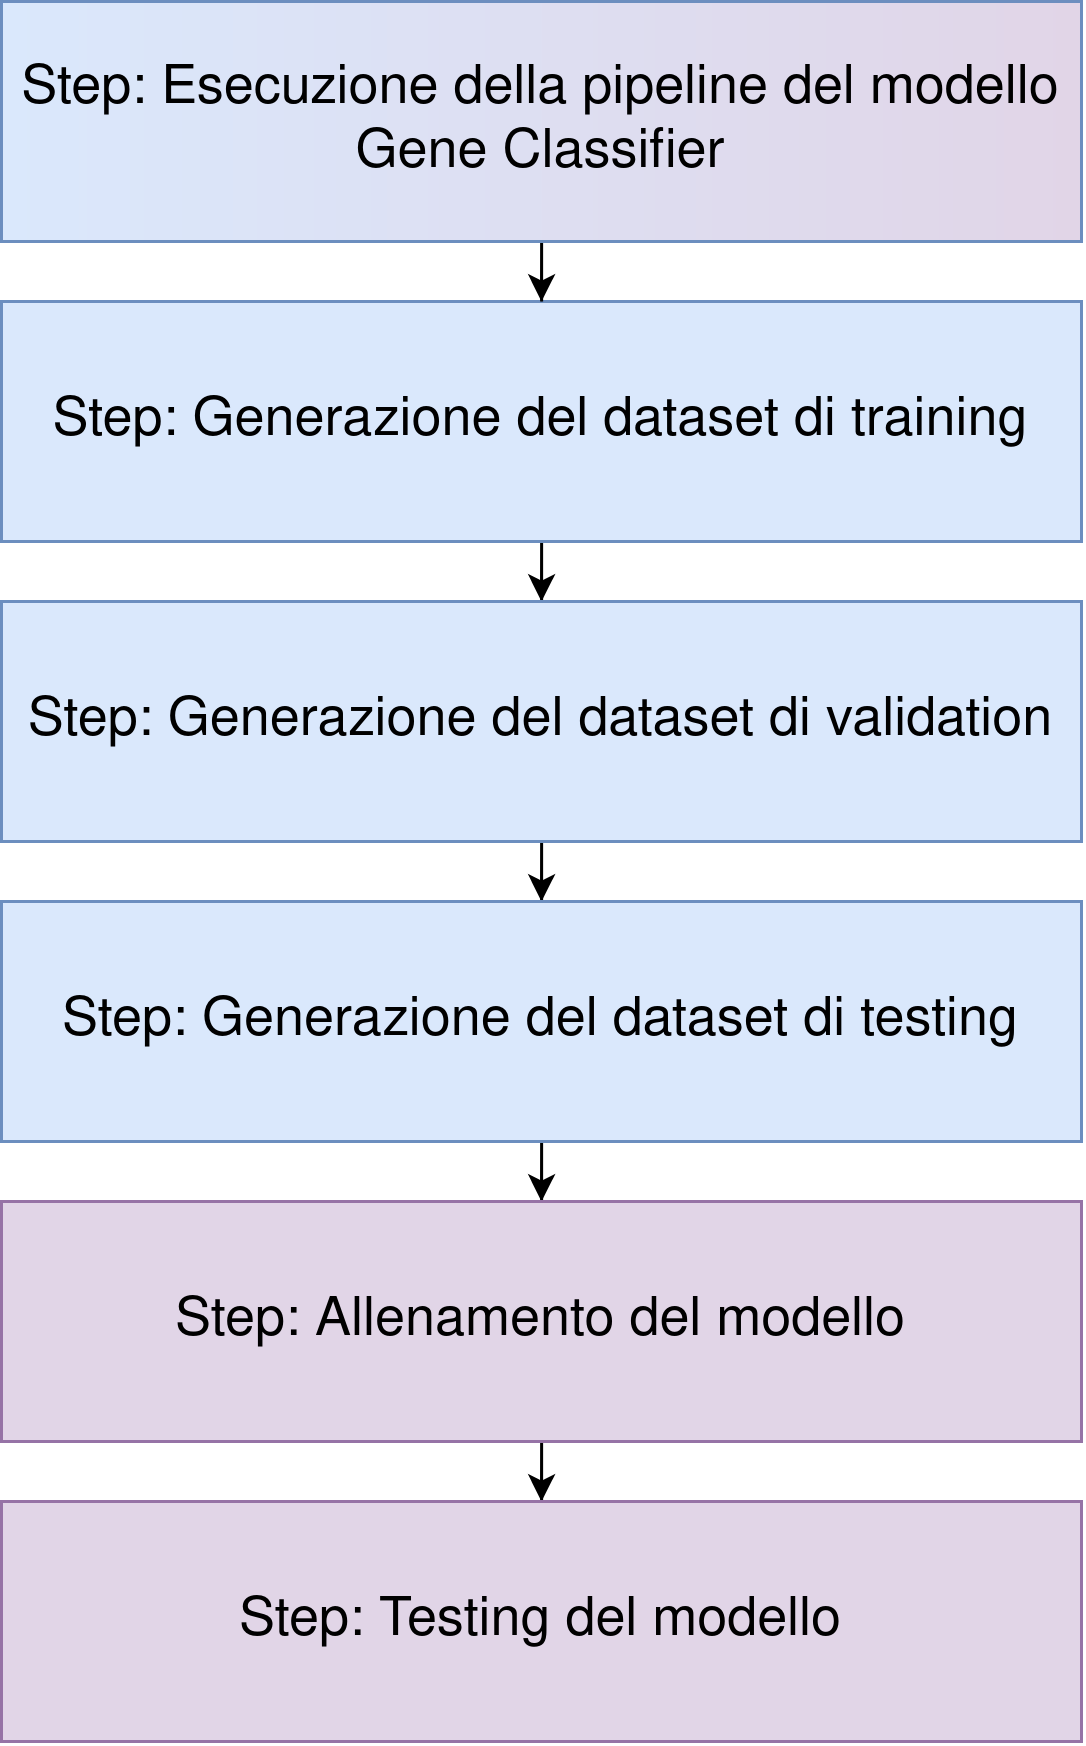
\includegraphics[width=150px]{figures/ch2/fusion_stati.png}
    \caption[Sequenza di operazioni del modello Fusion Classifier]{Sequenza di operazioni del modello Fusion Classifier}
    \label{fig:cha2:fusion_stati}
\end{figure}

Il modello Fusion Classifier permette di individuare la presenza di geni di fusione, sfruttando l'output del modello Gene Classifier per la classificazione delle fusioni genetiche.

Come per il modello Gene Classifier, i dati in input vengono suddivisi in training, testing e validation. L'output del modello Gene Classifier viene compattato in un unico input per il modello Fusion Classifier.

Viene impiegata una rete neurale {\em fully-connected} in cui il primo layer è un layer di protezione della dimensione dell'input, seguito da una serie di hidden layers completamente connessi e seguiti a loro volta da un layer di dropout per evitare l'overfitting. L'ultimo layer è il layer di classificazione, che restituirà in input la probabilità di appartenere alla classe delle sequenze chimeriche, cioè un valore booleano compreso fra 0 e 1.

Anche in questo caso, descrizioni più minuziose del funzionamento del modello sono disponibili nei lavori originali citati in precedenza.

\section{Ristrutturazione delle macchine a stati dei modelli}

Com'è possibile osservare dalle Figura 2.2 e 2.3, la natura sequenziale delle operazioni è una evidente limitazione che potrebbero fungere da collo di bottiglia per le performance dei modelli. E' inoltre chiaro come sia specialmente il modello Fusion Classifier a risentire negativamente della natura fortemente sequenziale della pipeline, nonché alla sua inerente struttura monolitica espressa dal singolo script Python che ne governa il funzionamento.

Si propone, quindi, una possibile ristrutturazione delle due macchine a stati.

\begin{figure}[h]
    \centering
    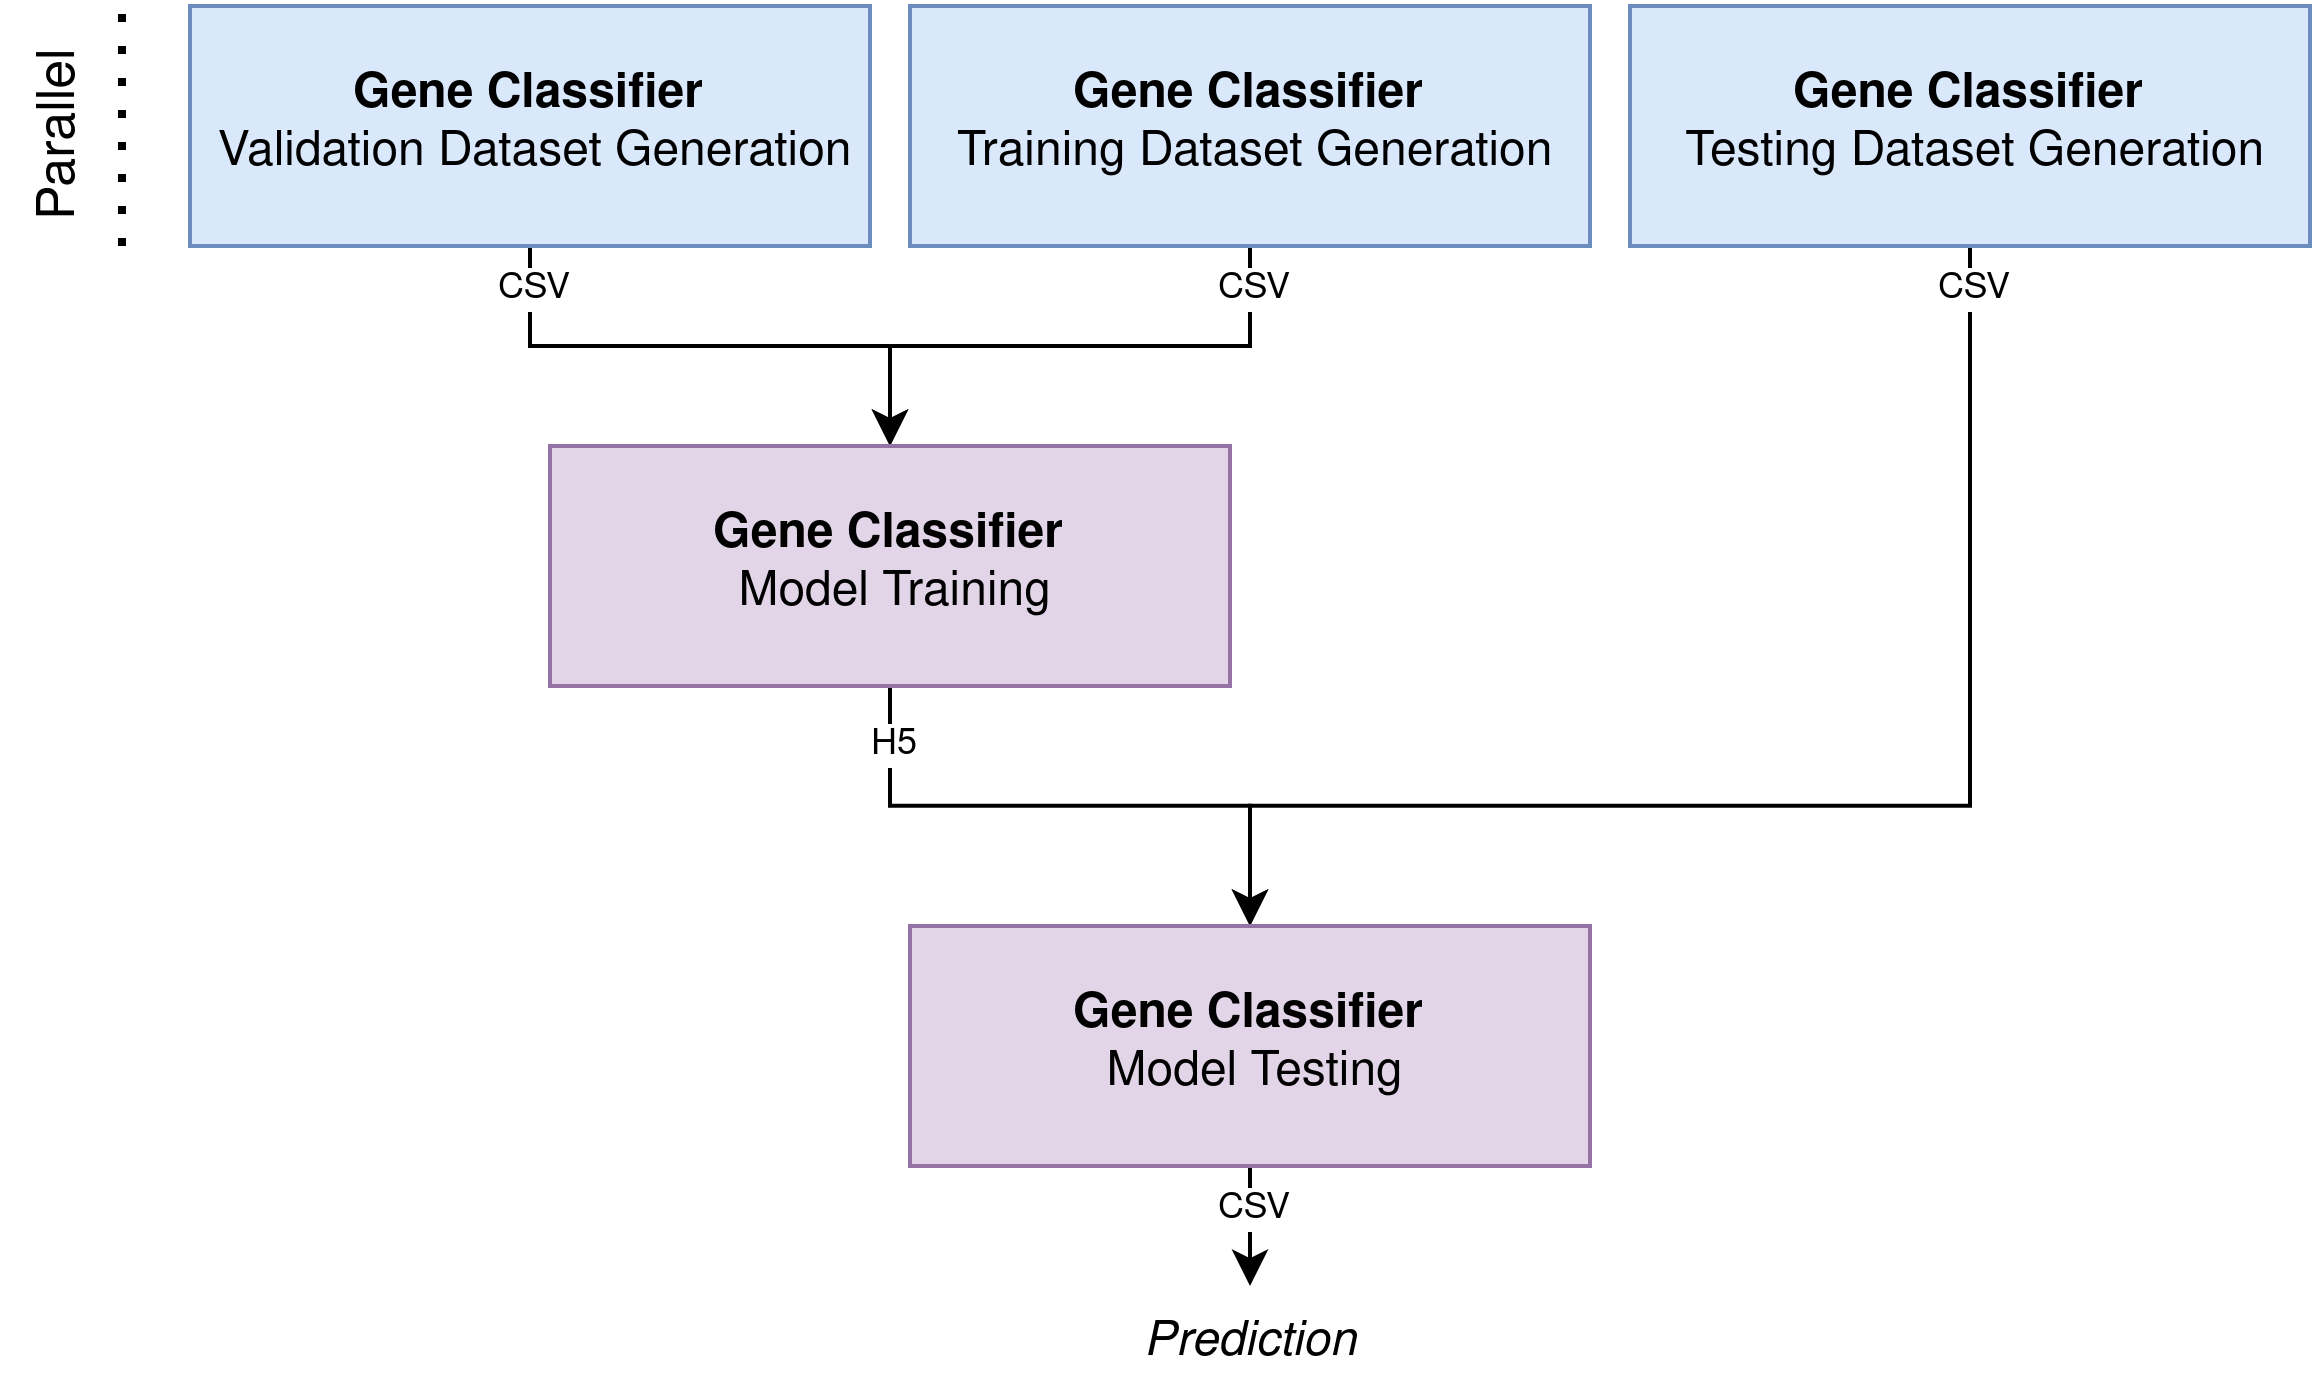
\includegraphics[width=\linewidth]{figures/ch2/new_gene.png}
    \caption[Ristrutturazione del modello Gene Classifier]{Ristrutturazione del modello Gene Classifier}
    \label{fig:cha2:new_gene_stati}
\end{figure}

Nella ristrutturazione del modello Gene Classifier, vengono parallelizzate le operazioni di generazione dei dataset di training, testing e validation. Il training sarà eseguito dopo la generazione dei dataset di training e validation; il testing, invece, sarà eseguito dopo il training e la generazione del dataset di testing.

\begin{figure}[h]
    \centering
    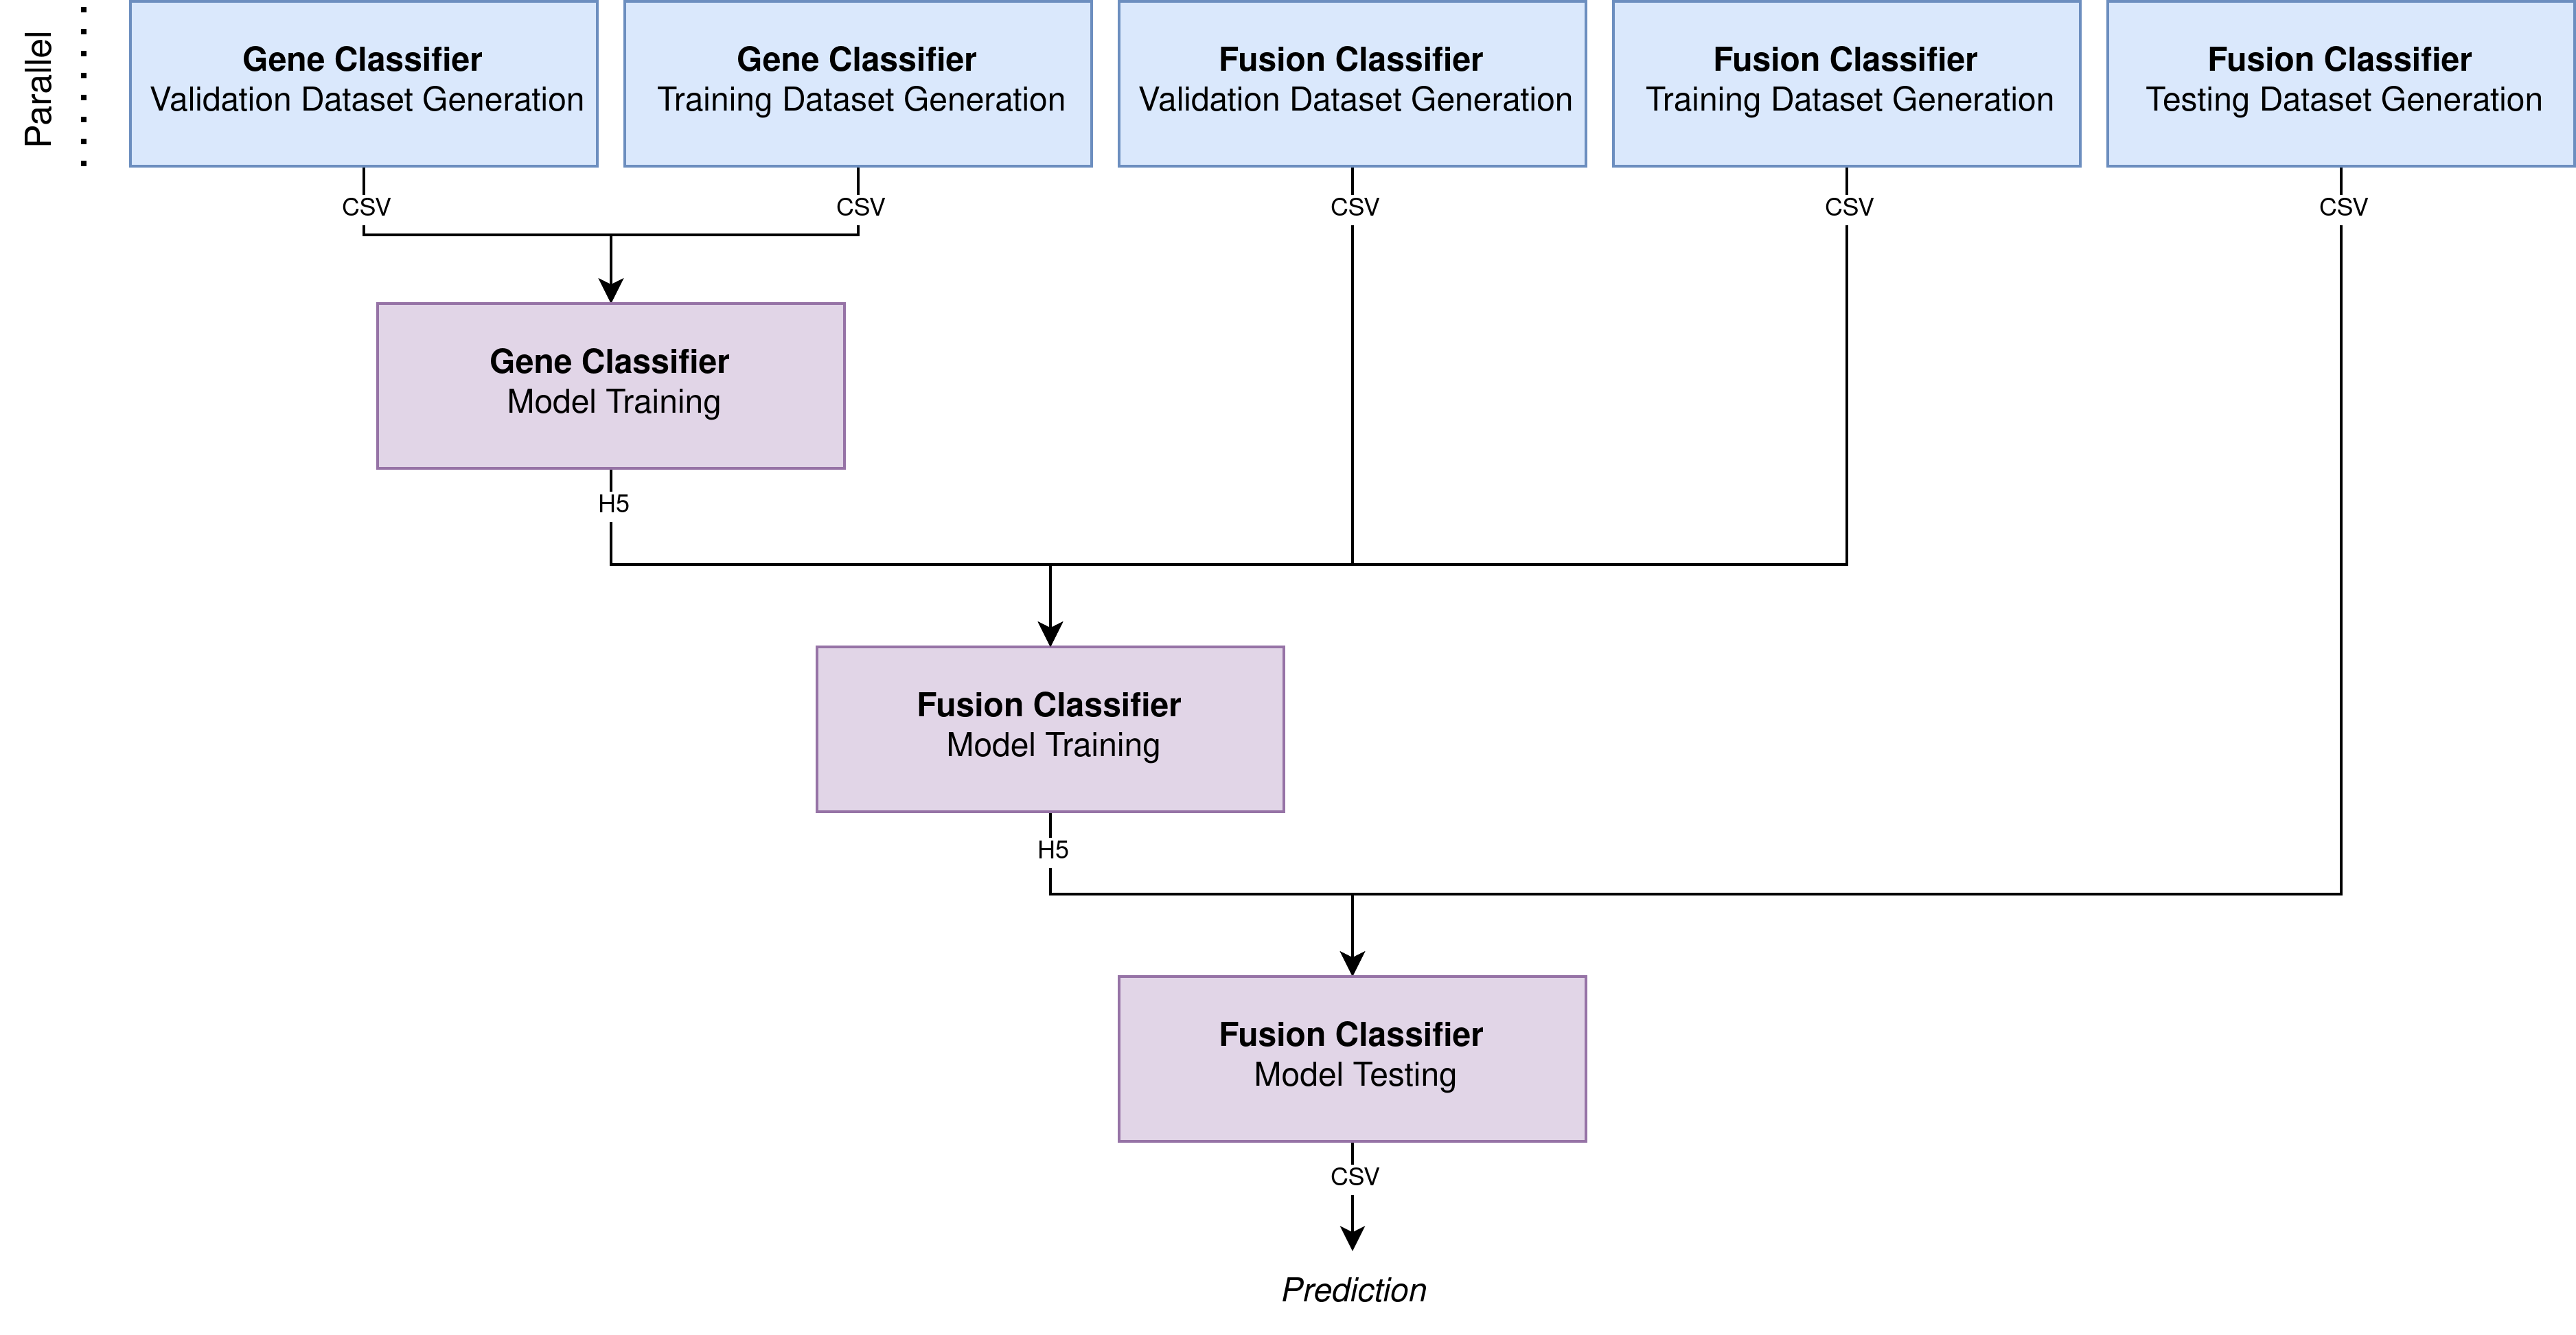
\includegraphics[width=\linewidth]{figures/ch2/new_fusion.png}
    \caption[Ristrutturazione del modello Fusion Classifier]{Ristrutturazione del modello Fusion Classifier}
    \label{fig:cha2:new_fusion_stati}
\end{figure}

Nella ristrutturazione del modello Fusion Classifier, vengono parallelizzate le operazioni di generazione dei dataset di training, testing e validation per il modello Fusion Classifier e, allo stesso tempo, vengono prodotti i dataset di validation e training del modello Gene Classifier. Il training del modello Fusion Classifier sarà eseguito dopo la generazione dei dataset di training e validation del modello Fusion Classifier, e dopo il training del modello Gene Classifier; il testing, invece, sarà eseguito dopo il training e la generazione del dataset di testing del modello Fusion Classifier.

\begin{figure}[h]
    \centering
    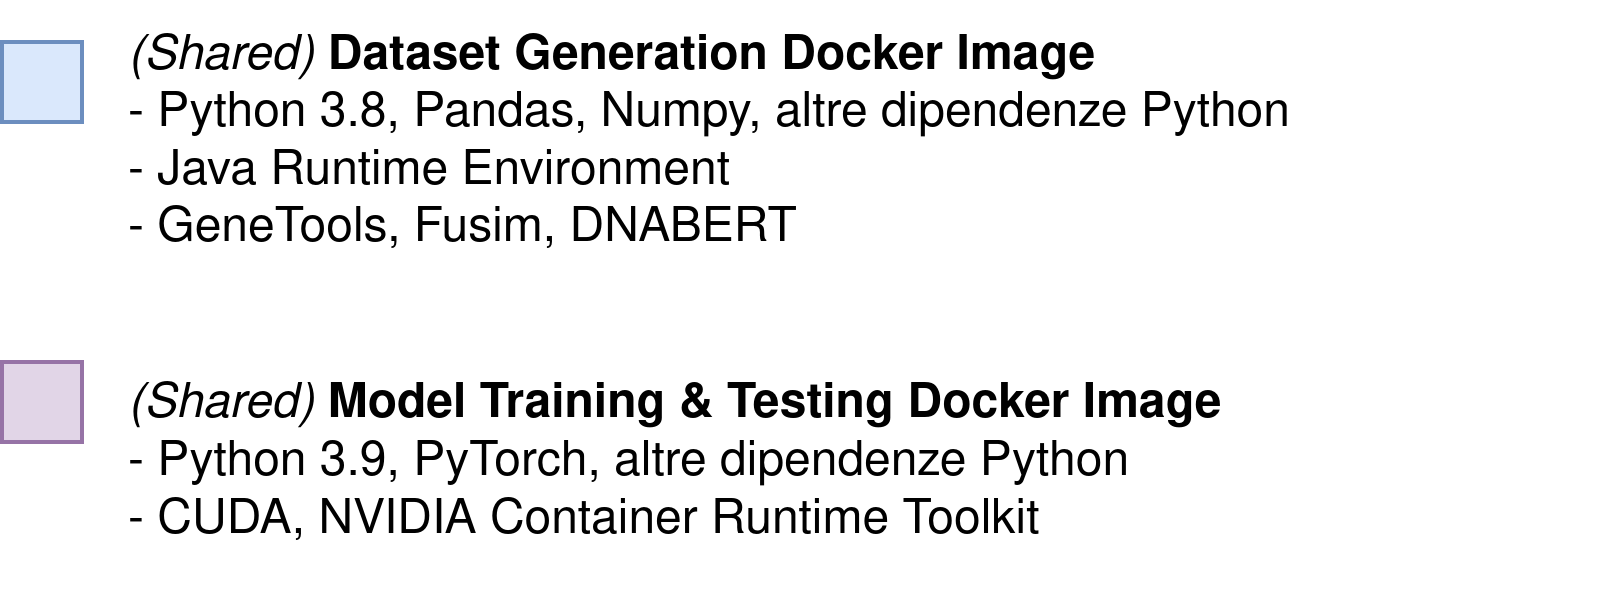
\includegraphics[width=300px]{figures/ch2/dependencies.png}
    \caption[Legenda dei microservizi]{Legenda dei microservizi}
    \label{fig:cha2:deps}
\end{figure}

Come inoltre indicato nel paragrafo 2.1, è possibile individuare dipendenze (in termini di moduli Python) individuali per specifici step delle macchine a stati. Intuitivamente, effettuare il training e il testing non ha le stesse esigenze tecnologiche rispetto alla generazione del dataset, e viceversa. Ergo, è possibile classificare gl stati in base alle loro dipendenze Python, e all'ambiente necessario per eseguire quei specifici step.

E' immediatamente osservabile una suddivisione in due potenziali \glsname{microservizi}, frammentando il precedente monolite.

In particolare, le macchine a stati si compongono delle seguenti tipologie di microservizi:

\begin{itemize}
    \item {\em Dataset Generation Microservice}
    \item {\em Model Training \& Testing Microservice}
\end{itemize}

La realizzazione di questi microservizi sarà descritta nei capitoli successivi, pur anticipando che la loro forma risultante sarà un container \glsname{docker} contenente le dipendenze del rispettivo servizio.

La problematica legata alla frammentazione in microservizi indipendenti giace nella necessità di {\em orchestrarli} al fine ultimo di ottenere lo stesso risultato raggiunto dall'architettura monolitica, sebbene con performance migliori.

Inoltre, la suddivisione in microservizi snelli e flessibili ci permette anche di rendere i modelli GeneFusion portabili su infrastrutture \glsname{cloudnative} e \glsname{bm} con estrema facilità, mediante tecniche di containerizazzione ben note. Ulteriori motivazioni a carico di questo approccio distribuito saranno esibite di seguito.